\documentclass[11pt]{article}

\usepackage{graphicx}
\usepackage{hyperref}
\usepackage{natbib}
\usepackage{amsmath}

\bibliographystyle{plain}
\setlength{\textwidth}{6.5in}
\setlength{\headheight}{0in}
\setlength{\textheight}{8.0in}
\setlength{\hoffset}{0in}
\setlength{\voffset}{0in}
\setlength{\oddsidemargin}{0in}
\setlength{\evensidemargin}{0in}


\title{Computational Physics -  Problem Set 8}
  
\author{Frederik Holst Knudsen}


\begin{document}

\maketitle
Github URL: https://github.com/frederikholst/phys-ga2000
\section{Maximization Likelihood Problem}
We want to maximize the Likelihood function:
$$L=\prod_{i=1}^{N} p(x_i)^{y_i}(1-p(x_i))^{1-y_i}$$
where the $y_i$'s are the answers of the survey and $p(x_i)$ is the PDF given in the problem:
$$p(x)=\frac{1}{1+\exp [-(\beta_0-\beta_1 x)]}$$.
To avoid large numbers, we minimize the negative log likelihood instead of Maximization:
$$\mathcal{L}=-\sum_{i=1}^{N}y_i \log (p(x_i)-(1-y_i)\log (1-p(x_i))) $$.
This way we get the fit shown in Figure \ref{fit}, with $\beta_0=-5$ and $\beta_1=0.09830074$. 
\begin{figure}[!htbp]
    \centering
    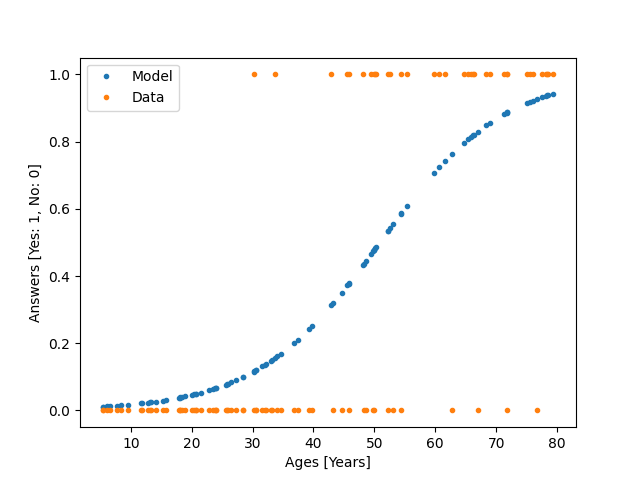
\includegraphics[width=0.7\textwidth]{fit.png}
    \caption{The logistic regression function p(x) fitted to the data of the survey with the parameters, $\beta_0=-5$ and $\beta_1=0.09830074$, which was found using Likelihood Maximization.   }
    \label{fit}
\end{figure}


The covariance matrix is found to be:
\[
\begin{bmatrix}
8.6736393 \times 10^{-1} & -1.6442016 \times 10^{-2} \\
-1.6442016 \times 10^{-2} & 3.4502562 \times 10^{-4}
\end{bmatrix}
\]

and the standard deviation is: 
$$STD_{\beta 0}= 0.931323766708374$$
$$STD_{\beta 1}= 0.01857486553490162$$.



\section{Newman 7.3: FFT of Trumpet and Piano}
In Figure \ref{fft1} we see the spectrum comparison of the piano and the trumpet playing the same note. The overtones of the trumpet is more prominent, giving rise the more sharper sounding instrument than that of the piano. Since the overtones andthe fundamental tone overlap, the two instruments are, however, playing the same note. 

\begin{figure}[!htbp]
    \centering
    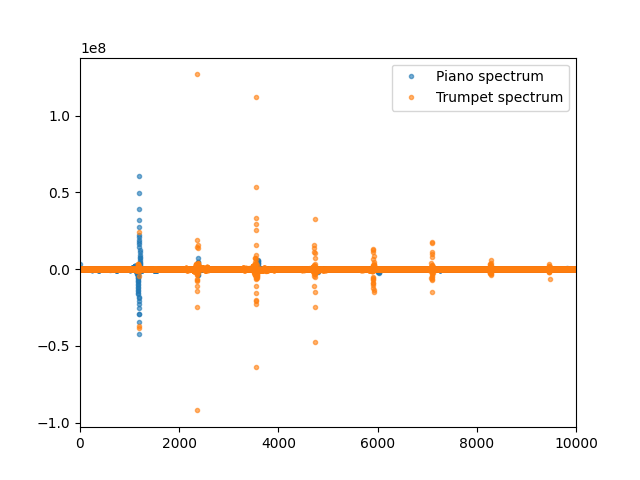
\includegraphics[width=0.7\textwidth]{pianotrumpet1.png}
    \caption{Here we see the side-by-side comparison of the spectrum of the two instruments. One notices the sharper overtones from the trumpet.}
    \label{fft1}
\end{figure}


To rescale the axis, we use that the sampling rate is 44100 samples per second. Scaling with the ratio of the sampling rate and the sample size, we obtain the units of frequency (1/s), see Figure \ref{C}. We find the index at the maximum of the spectra, and find the fundamental frequency, to be 525.231 Hz, so very likely the instruments played the fifth C (C5), an octave above the middle C.


\begin{figure}[!htbp]
    \centering
    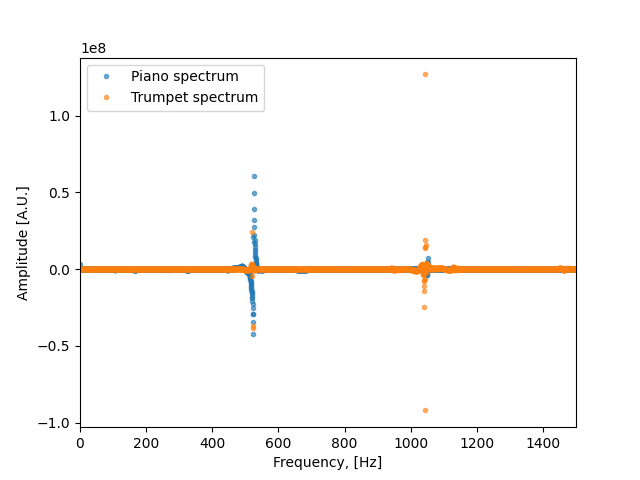
\includegraphics[width=0.7\textwidth]{C5.png}
    \caption{The fundamental tone and first overtone of the piano and trumpet with scaled axis in units of Hz.}
    \label{C}
\end{figure}



\section{Newman 7.4}
PART A: We load the dow-file and plot the data as seen in Figure \ref{dow}. 
\begin{figure}[!htbp]
    \centering
    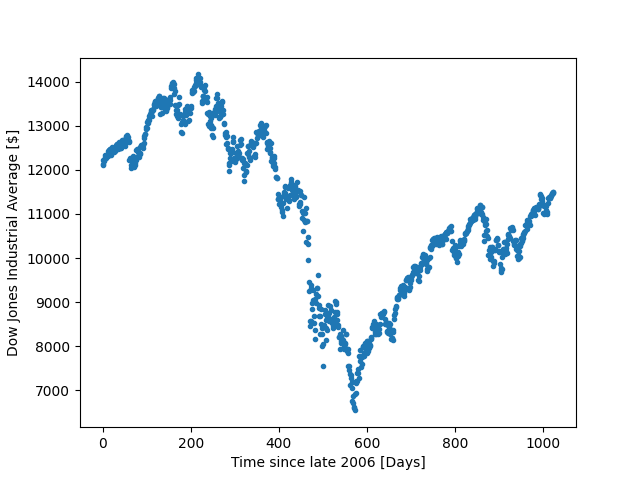
\includegraphics[width=0.7\textwidth]{dow.png}
    \caption{The Dow Jones Average from 2006 to 2010.}
    \label{dow}
\end{figure}

PART B: We calculate the coefficients of the discrete Fourier transform of the data using the numpy function np.fft.rfft.

PART C: We now set the first 10 percent of the elements of the coefficients to zero.

PARCT D: We carry out the inverse Fourier transform. See Figure \ref{high}
\begin{figure}[!htbp]
    \centering
    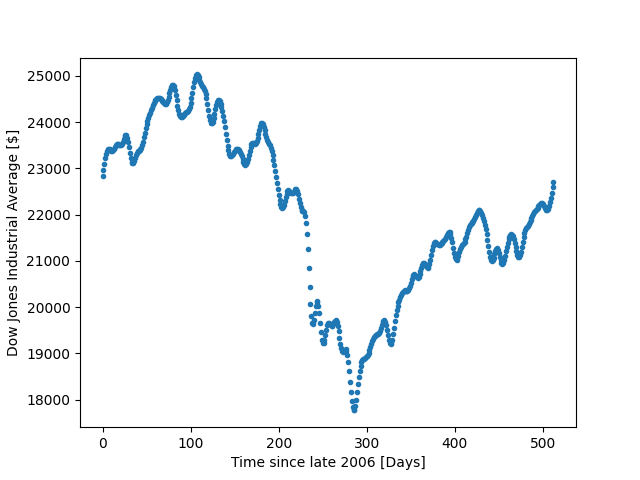
\includegraphics[width=0.7\textwidth]{high_cut.png}
    \caption{The Dow Jones Average from 2006 to 2010, but now with a low pass filter, by only letting the first 10 percent of the Fourier coefficients be nonzero. This is effectively removing the high oscillitating effects on the graph. }
    \label{high}
\end{figure}

PARCT E: Same as before, but now with an even stronger low pass, so it's only the first 2 percent of the coefficients that are nonzero. See Figure \ref{v high}.
\begin{figure}[!htbp]
    \centering
    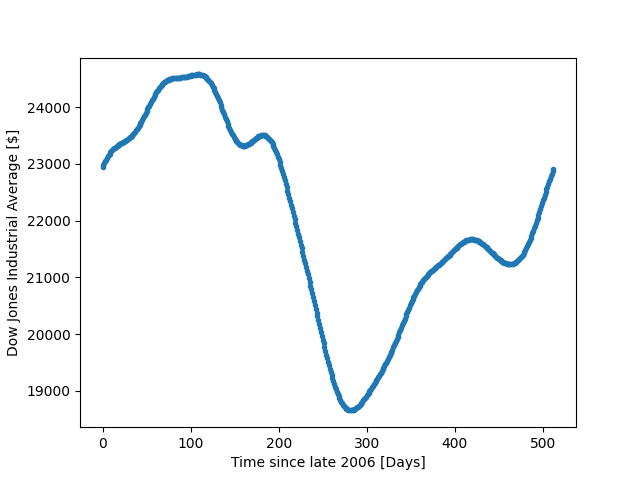
\includegraphics[width=0.7\textwidth]{v_high_cut.png}
    \caption{The Dow Jones Average from 2006 to 2010, but now with a stronger low pass filter, by only letting the lowest 2 percent of the Fourier coefficients be nonzero. }
    \label{v high}
\end{figure}





\end{document}